\documentclass{article}
\usepackage{graphicx} % new way of doing eps files
\usepackage{listings} % nice code layout
\usepackage[usenames]{color} % color
\usepackage{float}
\definecolor{listinggray}{gray}{0.9}
\definecolor{graphgray}{gray}{0.7}
\definecolor{ans}{rgb}{1,0,0}
\definecolor{blue}{rgb}{0,0,1}
% \Verilog{title}{label}{file}
\newcommand{\Verilog}[3]{
  \lstset{language=Verilog}
  \lstset{backgroundcolor=\color{listinggray},rulecolor=\color{blue}}
  \lstset{linewidth=\textwidth}
  \lstset{commentstyle=\textit, stringstyle=\upshape,showspaces=false}
  \lstset{frame=tb}
  \lstinputlisting[caption={#1},label={#2}]{#3}
}


\author{Jon Johnston and Justin Roessler}
\title{Lab4: Beginning to Decode}

\begin{document}
\maketitle

\section{Executive Summary}
The purpose of this lab is to create an Instruction Parse module that will break up the 32-bit instruction data into the R and D format cases. This module prepares an instruction to be executed and saves each part of an instruction according to its purpose (Rn,Rm,Rd, Opcode, etc.). Also, a Register File module was created in order to read and write information to registers. The regfile is the core memory of our processor. The Register File will read data from a read\_register location to send it out to the ALU. If RegWrite is set, it will write data from the ALU or memory to a write\_register location. After testing our files and analyzing the results, our lab was sucessful.
	

\section{Test Report}
To verify operation of these modules, this lab requires 2 test benches. 
\begin{enumerate}
	\item Instr\_Parse Test Bench
	\item RegFile Test Bench
\end{enumerate}

% This section should display the Expected Results Table and the Simulation Results for each test bench.  Make sure to label each figure correctly.  Please put them in the order of ERT1, SimResults1, ERT2, SimResults2 so that I can easily compare the ERT and Simulation Results.  To force the figures to be positioned correctly, add the float package (at the top of this file) and use the [H] after {figure} as I did below.  Also, if the ERT is on one page and the Simulation Results are on the next page, you can use a pagebreak as I did below so that the ERT goes to the next page also.

\pagebreak

\begin{figure}[H]
	\begin{center}
		\caption{Expected Results of the Instr\_Parse Test.}\label{fig:ert_Intsr_Parse_Test}
		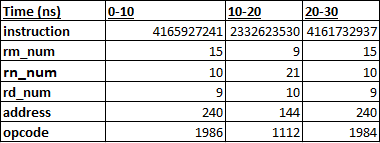
\includegraphics[width=1.0\textwidth]{../images/Instr_ParseExpected.png}
	\end{center}
\end{figure}

\begin{figure}[H]
	\begin{center}
		\caption{Timing diagram for the Instr\_Parse test.}\label{fig:Instr_Parse_Test}
		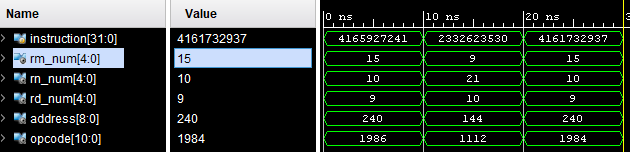
\includegraphics[width=1.0\textwidth]{../images/Instr_ParseSimulation.png}
	\end{center}
\end{figure}

\begin{figure}[H]
	\begin{center}
		\caption{Expected Results for the RegFile test.}\label{fig:ert_RegFile_Test}
		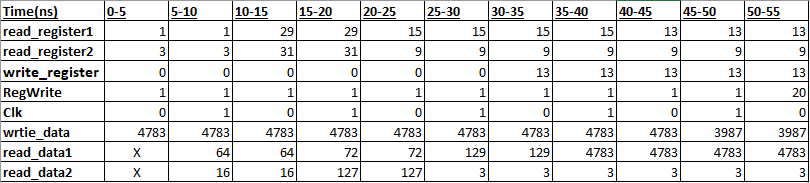
\includegraphics[width=1.0\textwidth]{../images/RegFileExpected.png}
	\end{center}
\end{figure}

\begin{figure}[H]
	\begin{center}
		\caption{Timing diagram for the RegFile test.}\label{fig:RegFile_Test}
		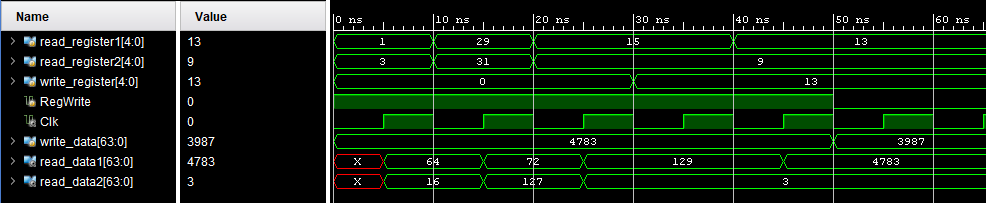
\includegraphics[width=1.0\textwidth]{../images/RegFileSimulation.png}
	\end{center}
\end{figure}

\pagebreak
\section{Code Appendix}
% The code appendix should include the test bench code and module code for this lab.
\Verilog{Verilog code for testing the instr\_parse\_test.}{code:regtest}{../code/2_decode/instr_parse_test.v}
\pagebreak
\Verilog{Verilog code for implementing the instr\_parse.}{code:reg}{../code/2_decode/instr_parse.v}
\Verilog{Verilog code for testing the regfile\_test.}{code:regtest}{../code/2_decode/regfile_test.v}
\Verilog{Verilog code for implementing the regfile.}{code:reg}{../code/2_decode/regfile.v}
\end{document} 